\documentclass[12pt]{article}
\usepackage{color}
\usepackage{floatrow}
\usepackage[margin=1in]{geometry}
\usepackage{listings}
\usepackage{setspace}
\usepackage{tikz}
\usepackage{graphicx}
\usepackage{subfig}


\definecolor{dkgreen}{rgb}{0,0.6,0}
\definecolor{gray}{rgb}{0.5,0.5,0.5}
\definecolor{mauve}{rgb}{0.58,0,0.82}

\setstretch{1}
\graphicspath{{images}}

\edef\restoreparindent{\parindent=\the\parindent\relax}
\usepackage{parskip}
\restoreparindent

\lstset{
  frame=tb,
  language=C++,
  aboveskip=3mm,
  belowskip=3mm,
  showstringspaces=false,
  columns=flexible,
  basicstyle={\small\ttfamily},
  numbers=none,
  numberstyle=\tiny\color{gray},
  keywordstyle=\color{blue},
  commentstyle=\color{dkgreen},
  stringstyle=\color{mauve},
  breaklines=true,
  breakatwhitespace=true,
  tabsize=3
}

\title{Mathematical Approach to an Optimal Algorithmic \textit{Snake} Game Agent}
\author{Malav Mehta}
\date{\today}

\begin{document}
\begin{singlespace}
\maketitle
\thispagestyle{empty}
\tableofcontents
\end{singlespace}

\clearpage
\setcounter{page}{1}
\pagebreak


\section{Introduction}

One of the primary focuses of mathematics is the modelling and optimization of real-life scenarios to automate processes or maximize desired results while minimizing use of resources. This field has countless practical applications in the realms of scientific, engineering, finance and algorithmic problems.

As an aspiring computer scientist, I have developed a particular interest in the intersection between math and programming. Alongside my passion for applied math, I also enjoy playing video games, being introduced to them after I first played the popular \textit{Snake} game on an old Nokia 3310 during my childhood. After taking the HL Math course, I started thinking about the things I regularly do from a mathematical point of view, so naturally, I decided to find a mathematically suitable way to create an efficient and autonomous agent for the \textit{Snake} game.

Hence, this investigation aims to find various \textbf{mathematical approaches to creating an optimal algorithmic \textit{Snake} game agent} and comparing them to conclusively determine the most efficient solution. For this investigation the most efficient algorithm will be the one which beats the game in the minimum amount of time. All approaches will be transformed into software agents for testing. This exploration will look at graph theory as a way to model the game and arrive at raw base approaches which will then be evaluated and combined with an analytical approach using probability density functions and calculus. 

\section{\textit{Snake} Game Mechanics}

The \textit{Snake} game is a very popular game, being first conceptualized in  the 1976 arcade game \textit{Blockade}. Since then, there have been hundreds of implementations of the game. It is thus important to define the rules of the version of the \textit{Snake} game that will be used in this exploration.

In the implementation that I have recreated in \texttt{C++} for this investigation (Figure \ref{fig:game_mechanics}), the autonomous agent controls a snake on the game plane. As the snake moves forward, left or right, it leaves a trail of fixed size behind it. The snake grows longer when its head runs into the apples and dies when it runs into itself or the borders. The objective is to grow long enough to cover the grid entirely, at which point the game is won.

\begin{figure}[!h]
\centering
\floatbox[{\capbeside\thisfloatsetup{capbesideposition={right,center},capbesidewidth=8cm}}]{figure}[\FBwidth]
	{\caption{The graphical representation of my implementation of the \textit{Snake} game. The \texttt{\makeatletter @\makeatother}, \texttt{\#} and red digit represent the snake's head, the snake's body and the apple, respectively} \label{fig:game_mechanics}
}
	{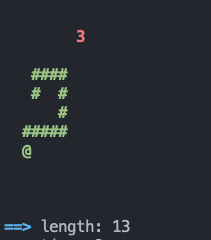
\includegraphics[scale=0.6]{game_mechanics.png}}
\end{figure}

\section{Modelling The Game}

While researching suitable models for representing the game, I came across graph theory, which is a branch in discrete mathematics. This was option topic 10 in last year's HL Math curriculum. In this section, I will explain what graph theory is, the notation that will be used in this exploration and how \textit{Snake} can be modelled by a graph.

\subsection{Graph Theory}

Graph theory refers to a way in which data can be represented. A  graph is a pair $G=(V,E)$ where $V$ is a set of vertices (also called nodes) and $E$ is a set of unordered pairs of vertices. The edge $e$ between vertices $v_{1}$ and $v_{2}$ is written as $e=v_{1}v_{2}=v_{2}v_{1}$. $v_{1}$ and $v_{2}$ are thus the endpoints of edge $e$ and are said to be adjacent to each other, written $v_{1} \leftrightarrow v_{2}$. A pair of vertices can be joined by at most one edge and no vertex can be joined to itself by an edge. For example, $G_{1}=(V_{1},E_{1})$ where $V_{1}=\{v_{1}, v_{2}, v_{3}\}$ and $E_{1}=\{v_{1}v_{2}, v_{2}v_{3}\}$ is drawn:

\begin{figure}[!h]
\centering
	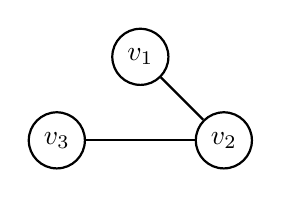
\begin{tikzpicture}[node distance={15mm}, main/.style={draw,circle}, thick]
		\node[main] (1) {$v_{1}$};
		\node[main] (2) [below right of=1] {$v_{2}$};
		\node[main] (3) [below left of=1] {$v_{3}$};

		\draw (1) to (2);
		\draw (2) to (3);
	\end{tikzpicture}
	\caption{Graph $G_{1}$}
	\label{fig:graph_g1}
\end{figure}

In graphs, there sometimes exist paths between two vertices and cycles containing multiple vertices. Formally, a graph $G_{p}=(V_{p}, E_{p})$ of $n$ vertices is a path from vertex $v_{1}$ to $v_{n}$ if $V_{p} = \{v_{1}, \ldots , v_{n} \}$ and $E_{p} = \{v_{i}v_{i+1} : i = 1, \ldots, n - 1\}$. $G_{p}$ is a cycle under the condition that $E_{p} = \{v_{i}v_{i+1} : i = 1, \ldots, n - 1\} \cup \{ v_{n}v_{1} \}$.

\subsection{Representing \textit{Snake} As A Graph}

To represent \textit{Snake} as a graph, it must first be visualized as a grid of width $m$ and height $n$ with $mn$ cells where each cell $c$ has coordinates $(x, y) : \{ 1 \leq x \leq m, 1 \leq y \leq n \}$ and the cell $c=(1,1)$ is on the top left of the grid (see Figure \ref{fig:snake_grid}).

\begin{figure}[!h]
\centering
	\def\arraystretch{1.5}
	\begin{tabular}{ | c | c | c | }
	\hline
	$(1, 1)$ & \ldots & $(m, 1)$ \\
	\hline
	\ldots &  & \ldots \\
	\hline
	$(1, n)$ & \ldots & $(m, n)$ \\
	\hline		
	\end{tabular}
	\caption{The \textit{Snake} game plane in grid format}
	\label{fig:snake_grid}
\end{figure}

Under this representation, the position of the snake and the apple can be represented as a set of cells and an individual cell, respectively. The snake can travel to cells that are adjacent to its head and are not already occupied by itself. To express this model as graph $G=(V,E)$ (see Figure \ref{fig:graph_g}), we can make the following considerations:

\begin{enumerate}
	\item Each cell $c$ can be represented as some 1vertex $v=(c_{x}, c_{y}) : \{ 1 \leq c_{x} \leq m, 1 \leq c_{y} \leq n \}$. The set of vertices $V$ of $G$ can thus be represented as $V=\{v_{i,j} : 1 \leq i \leq m, 1 \leq j \leq n \}$ where vertex $v_{i,j}$ refers to the cell at $(i,j)$.
	\item In the grid, the snake can travel to each cell non-diagonally adjacent to its head. We can express the ability to travel from one cell to another as an edge between the corresponding two vertices. Therefore, for all $v_{i,j} \in V$, there exists an edge between $v_{i,j}$ and $v_{i+1,j}$, $v_{i-1,j}$, $v_{i,j+1}$ and $v_{i,j-1}$ in $E$ of $G$ if these adjacent vertices are in $V$.
	\item The snake's body can be represented as a set of vertices $S$ containing the vertices occupied by the snake's body such that $S \subseteq V$.
	\item The snake head can be represented as some vertex $v_{i,j} \in V$, denoted $v_{h}$ for presentation.
	\item The apple can be represented as some vertex $v_{i,j} \in V$, denoted $v_{a}$ for presentation.
\end{enumerate}

\begin{figure}[!h]
\centering
	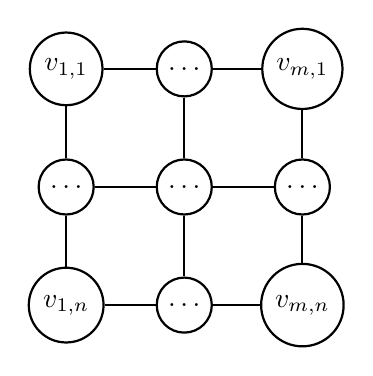
\begin{tikzpicture}[node distance={15mm}, main/.style={draw,circle}, thick]
		\node[main] (1) {$v_{1,1}$};
		\node[main] (2) [right of=1] {$\ldots$};
		\node[main] (3) [right of=2] {$v_{m,1}$};
		\node[main] (4) [below of=1] {$\ldots$};
		\node[main] (5) [below of=2] {$\ldots$};
		\node[main] (6) [below of=3] {$\ldots$};
		\node[main] (7) [below of=4] {$v_{1,n}$};
		\node[main] (8) [right of=7] {$\ldots$};
		\node[main] (9) [below of=6] {$v_{m,n}$};


		\draw (1) to (2);
		\draw (1) to (4);
		\draw (2) to (3);
		\draw (3) to (6);
		\draw (4) to (7);
		\draw (4) to (5);
		\draw (2) to (5);
		\draw (5) to (8);
		\draw (5) to (6);
		\draw (6) to (9);
		\draw (7) to (8);
		\draw (8) to (9);
	\end{tikzpicture}
	\caption{Graph $G$}
	\label{fig:graph_g}
\end{figure}

\section{Base Approaches}

The graph representation of the \textit{Snake} game represents the current state and models the positions of the snake and the apple on the game plane. Since the end goal is to be able to program the mathematical approach, a common way to implement mathematical logic is to have it isolated to a function where the information about the game state after each move is given as input and a suitable return value is outputted.

In the case of this exploration, the purpose of the function will be to find the best path that the snake should follow from its head in order to win the game. With this path generated, the first edge in the set of edges of the path contains the next vertex of where the snake head needs to go. Knowing this, the program can calculate the direction in which the snake must turn. Therefore, the return value should be the first edge of the best path.

\subsection{Breadth-First Search}

The most intuitive method for generating the best path with the goal of producing a time efficient mathematical approach is to compute the shortest path between the snake head and the apple. Returning the first edge of this path for each game state should be the quickest way for the snake to get to the apple, increase in size and eventually win the game.

A systematic approach for finding the shortest path between two vertices in a graph is to use the Breadth-First Search (BFS) algorithm. In the real-world, alongside other path-finding algorithms such as A-star and Dijkstra's, BFS is used in problems where exploring a graph is needed, such as for finding optimal flight routes between two cities. The BFS traversal of a graph terminates when every vertex of the graph has been visited. The concept is to visit all adjacent vertices of the starting vertex before visiting the vertices adjacent to the adjacent vertices. The algorithm takes the following steps:

\begin{enumerate}
	\item Keep a list of all vertices seen so far. Add the starting vertex to this list.
	\item Take the first vertex from the list, visit it and add unvisited adjacent vertices to the end of the list.
	\item Repeat the previous step until the list is empty.
\end{enumerate}

Consider Figure \ref{fig:graph_g2} with graph $G_{2} = (V_{2}, E_{2})$:

\begin{figure}[!h]
\centering
	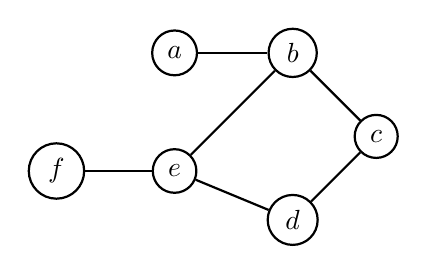
\begin{tikzpicture}[node distance={15mm}, main/.style={draw,circle}, thick]
		\node[main] (1) {$a$};
		\node[main] (2) [right of=1] {$b$};
		\node[main] (3) [below right of=2] {$c$};
		\node[main] (4) [below left of=3] {$d$};
		\node[main] (5) [below of=1] {$e$};
		\node[main] (6) [left of=5] {$f$};

		\draw (1) to (2);
		\draw (2) to (3);
		\draw (3) to (4);
		\draw (2) to (5);
		\draw (4) to (5);
		\draw (5) to (6);
	\end{tikzpicture}
	\caption{Graph $G_{2}$}
	\label{fig:graph_g2}
\end{figure}

Directly applying the BFS algorithm with starting vertex $a$, the traversal for the graph $G_{2}$ would be: $a \rightarrow b \rightarrow c \rightarrow e \rightarrow d \rightarrow f$. Rather than traversing all vertices, the application of BFS for the \textit{Snake} game problem requires finding the shortest path between the snake head and the apple. To accomplish this goal, we can modify the initial algorithm as such:

\begin{enumerate}
	\item Keep a list of vertices seen so far and the path required to get to the vertex as a pair. Add the pair of the starting vertex and an empty path to this list.
	\item Take the first pair from the list. This pair will have vertex $v$ and path $P$. Visit $v$ and for each unvisited vertex $u$ adjacent to $v$, duplicate path $P$ but also add edge $e = vu$ to it and finally add the pair $(u, \textrm{modified path } P)$ to the end of the list.
	\item Repeat the previous step until the end vertex is added to the list. If so, the associated path will be the shortest path from the starting vertex to the end vertex and return this path.
	\item If the list is empty before the end vertex is reached, return an empty path.
\end{enumerate}

Applying this modified BFS algorithm to $G_{2} $ with starting vertex $a$ and end vertex $e$, we see that the edges of the generated path are correctly $\{ab, be\}$ rather than $\{ab, bc, cd, de\}$. Therefore, this algorithm is suitable for finding the aforementioned best path for the snake to take under the shortest path approach.

To apply BFS to the \textit{Snake} game, we set $v_{h}$ as the starting vertex and $v_{a}$ as the end vertex. One final modification to make, to ensure that the generated path does not involved the snake head running into its body, is to add the following rule to step 2 from the modified algorithm: only adjacent vertices $u$ that are not already occupied by the snake's body should be added to the list. The final code for this approach is shown in Figure \ref{fig:bfs_code} of Appendix \ref{sec:appendix_code}.

Despite being a very quick solution and seemingly sound at first glance, a more comprehensive examination of the shortest path approach reveals a major flaw. Since the BFS algorithm is a greedy solution to the problem, in that it finds the best move for the current state and performs it without thinking of the consequences, it is not able to foresee the position of the snake after it has moved along the shortest path and thus traps itself. After running 100 000 simulations with this approach, it was never successful at beating the game. Each game ends in the ways shown in Figure \ref{fig:bfs_issues}.

\begin{figure}[!h]
\centering
	\subfloat[The apple gets enclosed by the snake]{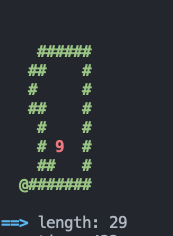
\includegraphics[scale=0.6]{circled_apple.png}\label{fig:bfs_issues_apple}}
	\hspace{1.15em}
	\subfloat[The snake traps itself along the border]{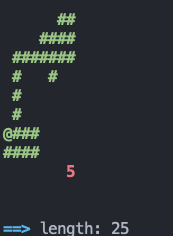
\includegraphics[scale=0.6]{circled_self.png}\label{fig:bfs_issues_self}}
	\caption{Lost scenarios with the BFS approach}
	\label{fig:bfs_issues}
\end{figure}

\subsection{Hamiltonian Cycle}

To remedy the flaw in the BFS approach, I decided to focus on a solution that would guarantee a win even if it meant that it might not be efficient time-wise. In my research, I watched videos of players winning \textit{Snake}. Although at first these players would take a greedy shortest path approach, they changed their strategy once the snake got longer, instead sticking to one fixed path and following it endlessly. Essentially, they traverse the game plane such that they visit every point exactly once before returning to the starting point and then repeating this loop. This can be recognized as a Hamiltonian cycle (also called a Hamiltonian circuit), formally defined to be a closed loop on a graph where each vertex is visited exactly once. Consider Figure \ref{fig:graph_g3} with graph $G_{3} = (V_{3}, E_{3})$:

\begin{figure}[!h]
\centering
	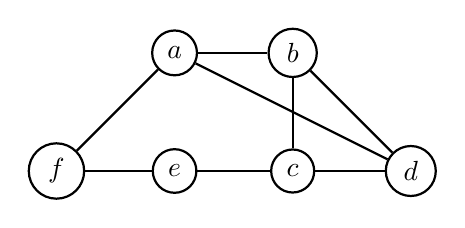
\begin{tikzpicture}[node distance={15mm}, main/.style={draw,circle}, thick]
		\node[main] (1) {$a$};
		\node[main] (2) [right of=1] {$b$};
		\node[main] (3) [below of=2] {$c$};
		\node[main] (4) [right of=3] {$d$};
		\node[main] (5) [below of=1] {$e$};
		\node[main] (6) [left of=5] {$f$};

		\draw (1) to (2);
		\draw (1) to (6);
		\draw (2) to (3);
		\draw (3) to (4);
		\draw (1) to (4);
		\draw (2) to (4);
		\draw (3) to (5);
		\draw (5) to (6);
	\end{tikzpicture}
	\caption{Graph $G_{3}$}
	\label{fig:graph_g3}
\end{figure}

$G_{3}$ is said to be Hamiltonian since there is a Hamiltonian cycle starting from vertex $a$: $a \rightarrow b \rightarrow d \rightarrow c \rightarrow e \rightarrow f \rightarrow a$. The rationale behind having the snake follow a Hamiltonian cycle is that no matter where it goes, it will never be able to trap itself since it will not be able to run into itself until the entire graph consists only of the snake. Thus, it is guaranteed that an agent based on this approach will win the game.

However, in order for the graph $G$ which represents the $Snake$ game plane to be Hamiltonian, the width of $m$ and height $n$ of this vertex grid must exist such that:

\begin{itemize}
	\item $m>1$, $n>1$ and either $m$ or $n$ is even. These constraints can be proved to work with a proof by construction. First, if $m=2$ or $n=2$ then a Hamiltonian cycle can be constructed by forming a ring that reaches all vertices.
	
If this is not the case, then there must exist a side in the grid with an even number of vertices greater than 2. We will call this direction \textit{vertical} (meaning that the graph will have an even number of rows) and the other direction \textit{horizontal}. Start from the first column of the first row and begin the path by extending it to the last column of this first row. Go one row down and return to the second column. If this is the last row of the graph, then further extend the path to the first column and connect it back to the vertex on the first column of the first row. If this is not the last row, then stay on the second column, drop one column down and repeat the initial process. Since there are an even number of rows, there will be exactly $n \over 2$ repetitions. Note that as long as $m > 2$ ($m = 2$ case considered above), the length of $m$ does not matter.

Therefore, it is always possible to construct a Hamiltonian cycle when $m>1$, $n>1$ and either $m$ or $n$ is even. See Figure \ref{fig:cycle_proof} for a visual example of the above proof.

\begin{figure}[!h]
\centering
	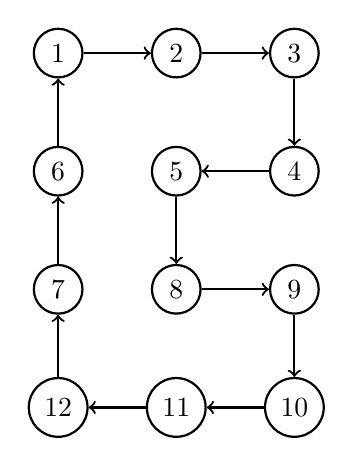
\begin{tikzpicture}[node distance={15mm}, main/.style={draw,circle}, thick]
		\node[main] (1) {1};
		\node[main] (2) [right of=1] {2};
		\node[main] (3) [right of=2] {3};
		\node[main] (4) [below of=3] {4};
		\node[main] (5) [left of=4] {5};
		\node[main] (6) [left of=5] {6};
		\node[main] (7) [below of=6] {7};
		\node[main] (8) [right of=7] {8};
		\node[main] (9) [right of=8] {9};
		\node[main] (10) [below of=9] {10};
		\node[main] (11) [left of=10] {11};
		\node[main] (12) [left of=11] {12};

		\draw[->] (1) to (2);
		\draw[->] (2) to (3);
		\draw[->] (3) to (4);
		\draw[->] (4) to (5);
		\draw[->] (5) to (8);
		\draw[->] (8) to (9);
		\draw[->] (9) to (10);
		\draw[->] (10) to (11);
		\draw[->] (11) to (12);
		\draw[->] (12) to (7);
		\draw[->] (7) to (6);
		\draw[->] (6) to (1);
		
	\end{tikzpicture}
	\caption{Numbered Hamiltonian cycle of grid graph for $m=3$ and $n=4$}
	\label{fig:cycle_proof}
\end{figure}

	
	\item \textbf{Or} $mn = 1$. Under this scenario, the graph contains only one vertex and is trivially Hamiltonian with a zero length path that visits the vertex.
\end{itemize}

If only one of $m$ and $n$ are equal to 1, then the graph is a straight line. In this case, it is impossible to form a Hamiltonian cycle. If both $m$ and $n$ are odd and $mn$ is not equal to 1, then we have a bipartite graph with unbalanced vertex parity, which, by Grinberg's Theorem, is known to not be Hamiltonian.

To implement this idea in code as an autonomous agent, the most efficient solution would be to generate a Hamiltonian cycle for the game graph when the game is first initialized. This way, the function into which the game state would be the input already has the best path for the snake in memory and the code can check where the snake head is to determine where it should turn next.

Note that generating a Hamiltonian cycle is an NP (non-polynomial time) hard problem in computation, since there are $\frac{1}{2} (n-1)!$ candidate cycles in any graph with $n$ vertices. Instead, I used a heuristic proposed by Chuyang Liu (see code on Figure \ref{fig:cycle_code} of Appendix \ref{sec:appendix_code}). After making this implementation, as can be seen in Figure \ref{fig:finished_cycle} the game can now be solved.

\begin{figure}[!h]
\centering
	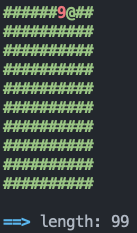
\includegraphics[scale=0.6]{finished_cycle.png}
	\caption{Completed game for a $10 \times 10$ grid}
	\label{fig:finished_cycle}
\end{figure}

While this is a valid approach to solving the game, it does not address the needs outlined in the aim of this investigation of developing an \textbf{optimal} approach: one requiring a minimum amount of time. At the beginning of the game, when the length of the snake is only one, the snake head may need to move up to $mn - 1$ turns before reaching the apple in the worst case scenario. On average, at length $l$, the snake needs to move for $\frac{1}{2} (mn-l)$ turns before reaching the apple. Therefore, this is an extremely slow approach and is thus not the ideal way to mathematically solve the game.

\section{Analytical Approach}

Despite their shortcomings, both the BFS and Hamiltonian cycle approaches had their strengths. For a grid where $m=n=10$, the agent using the BFS approach experimentally survived until the length of the snake was over 20. Notably, it got to this length very quickly using its greedy shortest path approach. The Hamiltonian cycle on the other hand, despite being a slower approach, always guaranteed that the game would be won.

Referring back to the method that human players took to beat the game, we can observe that a combination of the two aforementioned base approaches will be the most optimal. A final approach, in which both of these solutions are combined, will be enhanced by both of their benefits. To model the human players, the third approach will first begin with BFS followed by a conversion to the Hamiltonian cycle after some length. The most critical aspect with this approach is to determine what length maximizes the benefits of the speed of BFS in order to minimize the time but also assures survival of the snake. To find this length, I can optimize using differential calculus a function $T$  where $T(l)$ represents the total amount of moves (or turns including going straight) that will be taken if the models switches from BFS to the Hamiltonian cycle at length $l$.

\subsection{Probabilistic Modelling}



\subsection{Optimization}

\section{Evaluation}

\subsection{Comparison}

\subsection{Reflection}

\section{Conclusion}

\pagebreak
\begin{thebibliography}{9}
\bibitem{latexcompanion} 
Michel Goossens, Frank Mittelbach, and Alexander Samarin. 
\textit{The \LaTeX\ Companion}. 
Addison-Wesley, Reading, Massachusetts, 1993.

\bibitem{einstein} 
Albert Einstein. 
\textit{Zur Elektrodynamik bewegter K{\"o}rper}. (German) 
[\textit{On the electrodynamics of moving bodies}]. 
Annalen der Physik, 322(10):891–921, 1905.

\bibitem{knuthwebsite} 
Knuth: Computers and Typesetting,
\\\texttt{http://www-cs-faculty.stanford.edu/\~{}uno/abcde.html}
\end{thebibliography}
\pagebreak


\appendix
\section{C++ Code}\label{sec:appendix_code}

\begin{figure}[!h]
\centering
\begin{lstlisting}
vector<Node> shortest_path(Node des) {
    queue<vector<Node> > q{{snake.back()}};
    vis.clear();
    for (Node u : snake)
      vis[u] = 1;
    vis[des] = 0;
    
    while (!q.empty()) {
      vector<Node> path = q.front();
      q.pop();
     
      if (path.back() == des)
        return path;
        
      for (Node u : path.back().adj()) {
        if (is_valid(u) && !vis[u]) {
          vis[u] = 1;
          vector<Node> new_path(path);
          new_path.push_back(u);
          q.push(new_path);
        }
      }
    }
    return {};
}
\end{lstlisting}
\caption{Code for performing a \textbf{Breadth-First Search}.}
\label{fig:bfs_code}
\end{figure}

\begin{figure}[!h]
\begin{lstlisting}
void build_cycle() {
    cycle.clear();
    vector<Node> path_dir = longest_path(snake[0]), snake_path = dir_path(snake);
    for (Node u : snake_path)
      path_dir.push_back(u);
    Node cur = snake.back();
    for (Node u : path_dir) {
      cycle[cur] = u;
      cur = cur + u;
    }
    cycle_size = path_dir.size();
}
\end{lstlisting}
\caption{Code for generating a \textbf{Hamiltonian Cycle} (heuristic).}
\label{fig:cycle_code}
\end{figure}

\end{document}